\documentclass{article}
\usepackage{epsfig, latexsym}

\begin{document}

\newcommand{\SOPmin}{${\rm SOP}_{\rm min} \ $}
\newcommand{\POSmin}{${\rm POS}_{\rm min} \ $}
\newcommand{\bs}{\backslash}
\newcommand{\x}{\addtocounter{enumi}{1} \theenumi}


\title{
\Huge{CSE 271}\\
\normalsize{Exam 3}\\
\normalsize{Return this document!!!}\\
\makebox[4in][l]{Name:}
SSN:}
\date{}

\maketitle{}

\begin{enumerate}
\item {\bf (3 pts.)} How many different \SOPmin realizations does F have?
F(A,B,C,D)=$\Sigma$m(3,4,5,7,8,9,11,12)

$$ \begin{array} {c||c|c|c|c}
        AB \bs CD & 00 & 01 & 11 & 10 \\ \hline \hline
        00        &    &    &    &    \\ \hline
        01        &    &    &    &    \\ \hline
        11        &    &    &    &    \\ \hline
        10        &    &    &    &    \\
\end{array} $$ 

\begin{tabular}{p{0.75in}p{0.75in}p{0.75in}p{0.75in}p{0.75in}}
a) 1 & b) 2 & c) 3 & d) 4 & e) 5 or more \\
\end{tabular}

\item {\bf (3 pts.)} The output of a sequential circuit is fundamentally
different than a combinational circuit because its output is a function
of the?
\begin{description}
\item{a) } State
\item{b) } Input
\item{c) } Output
\item{d) } Number of inputs
\item{e) } The staple monkey
\end{description}

\item {\bf (2 pts.)} You are told to implement a 3 bit counter using our seven
step FSM design process.  Each state represents the current count value.  The
state assignment is performed using a dense encoding. 
How many flip flops will this FSM require?

\begin{tabular}{p{0.75in}p{0.75in}p{0.75in}p{0.75in}p{0.75in}}
a) 3 & b) 4 & c) 7 & d) 8 & e) 16 \\
\end{tabular}

\item {\bf (2 pts.)} You are told to implement a 3 bit counter using the
ones hot design process.  Each state represents the current count value. 
How many flip flops will the counter require?

\begin{tabular}{p{0.75in}p{0.75in}p{0.75in}p{0.75in}p{0.75in}}
a) 3 & b) 4 & c) 7 & d) 8 & e) 16 \\
\end{tabular}

\pagebreak
\item {\bf (2 pts.)} Given the following state table and the state assignment,
determine the entry in the transition kmap marked with a *.
{\small
$$\begin{array}{lll}
$$\begin{array}{c||c|c}
        cs \bs X & 0   &  1  \\ \hline \hline
        A        & B,0 & A,0 \\ \hline
        B        & D,0 & A,0 \\ \hline
        C        & C,1 & B,1 \\ \hline
        D        & A,1 & C,1 \\ 
\end{array}$$
&
$$\begin{array}{c||c|c}
        state & Q_1 & Q_0    \\ \hline \hline
        A     & 1 & 0  \\ \hline
        B     & 0 & 0 \\ \hline
        C     & 1 & 1 \\ \hline
        D     & 0 & 1 \\
\end{array}$$
&
$$\begin{array}{c||c|c}
        Q_1 Q_0 \bs X & 0   &  1   \\ \hline \hline
        00       &     &     \\ \hline
        01       &     &     \\ \hline
        10       & *   &     \\ \hline
        11       &     &     \\
\end{array}$$\\
\end{array}$$}

\begin{description}
\item{a) }00,0
\item{b) }01,1
\item{c) }10,0
\item{d) }11,0
\item{e) }None of the above.
\end{description}

Given the transition kmap to the right, determine the MIEs
and OEs.
{\small
$$\begin{array}{cll}
$$\begin{array}{c||c|c|c|c}
        Q \bs X_1 X_0 & 00  & 01  & 11  & 10  \\ \hline \hline
        0             & 1,1 & 1,1 & 0,1 & 0,1 \\ \hline
        1             & 1,0 & 0,0 & 0,0 & 1,0 \\
\end{array}$$
&
$$\begin{array} {c||c|c|c|c}
        Q \bs X_1 X_0 & 00 & 01 & 11 & 10 \\ \hline \hline
        0             &    &    &    &    \\ \hline
        1             &    &    &    &    \\
\end{array}$$
&
$$\begin{array} {c||c|c|c|c}
        Q \bs X_1 X_0 & 00 & 01 & 11 & 10 \\ \hline \hline
        0             &    &    &    &    \\ \hline
        1             &    &    &    &    \\
\end{array}$$ \\
Q^+,Z & D= & Z= \\
\end{array}$$}
\item {\bf (2 pts.)} What does $D=$ ?
\begin{description}
\item{a) }$X_1'X_0' + Q'X_1' + QX_1X_0'$
\item{b) }$X_1'X_0' + Q'X_1' + QX_0'$
\item{c) }$Q'X_1' + QX_1X_0'$
\item{d) }$Q'X_1' + QX_0'$
\item{e) }$Q'$
\end{description}

\item {\bf (2 pts.)} What does $Z=$ ?
\begin{description}
\item{a) }$X_1'X_0' + Q'X_1' + QX_1X_0'$
\item{b) }$X_1'X_0' + Q'X_1' + QX_0'$
\item{c) }$Q'X_1' + QX_1X_0'$
\item{d) }$Q'X_1' + QX_0'$
\item{e) }$Q'$
\end{description}


\pagebreak
Questions 8-11 concern the FSM realization of the state diagram given below.
Assume a ones hot encoding of the states.  Call the input $X$ and the output
$Z$.  Let $D_A$ be the input to the flip flop representing state $A$.  Let $Q_A$
be the output from the flip flop representing state $A$.  Apply the preceding
definitions to $D_B, Q_B, D_C, Q_C$.

\item {\bf (1 pts.)} How many flip flops are required to realize this FSM?

\begin{tabular}{p{0.75in}p{0.75in}p{0.75in}p{0.75in}p{0.75in}}
a) 1 & b) 2 & c) 3 & d) 4 & e) 5 \\
\end{tabular}

\item {\bf (3 pts.)} What is the memory input equation for flip flop $A$?
\begin{description}
\item{a) } 1
\item{b) } 0
\item{c) } $X'Q_B$
\item{d) } $XQ_A + XQ_C$
\item{e) } None of the above.
\end{description}

\item {\bf (3 pts.)} What is the memory input equation for flip flop $R$?
\begin{description}
\item{a) } 1
\item{b) } 0
\item{c) } $XQ_B + X'Q_C$
\item{d) } $Q_R$
\item{e) } None of the above.
\end{description}
\includegraphics[-60mm,15mm][0mm,15.1mm]{./Fig3/sd.eps}
\item {\bf (3 pts.)} What is the equation for $Z$?
\begin{description}
\item{a) } 0
\item{b) } 1
\item{c) } $Q_R$ + $Q_C$
\item{d) } $XQ_R + XQ_C + XQ_B + XQ_A$
\item{e) } None of the above.
\end{description}

\pagebreak

\pagebreak
For questions 12-14 assume that you have constructed a circuit
which is involved in a 2-line handshake; your circuit
is a passive consumer of data.  

\item {\bf (3 pts.)} Which of the following explanations justifies 
waiting for the request to be lowered before processing the data?
\begin{description}
\item{a) } The external world may be much faster than your circuit.
\item{b) } The external world may be much slower than your circuit.
\item{c) } The external world may be the same speed as your circuit.
\item{d) } The external world may be busy.
\item{e) } Our circuit may be busy.
\end{description}

\item {\bf (3 pts.)} Which of the following explanations justifies asserting
an acknowledgement after you latch the data?
\begin{description}
\item{a) } The external world may be much faster than your circuit.
\item{b) } The external world may be much slower than your circuit.
\item{c) } The external world may be the same speed as your circuit.
\item{d) } The external world may be busy.
\item{e) } Our circuit may be busy.
\end{description}

\item {\bf (3 pts.)} What role does the external world play in the 
2-line handshake?
\begin{description}
\item{a) } Active producer
\item{b) } Passive producer
\item{c) } Active consumer
\item{d) } Passive consumer
\end{description}


\pagebreak
For questions 15-220use the state diagram below.  Assume that the
FSM is built correctly.  The symbols $a,b,A,B,C$ are standing in for
the actual variables that have been placed on the arcs (I am using
these symbols to hide their actual values).  This question requires
you to think about the potential variables that could appear on the 
arcs of a legally built FSM.  Mark Always if all legal expressions
on the arcs satisfy the stated condition. Mark Sometimes if some,
but not all, legal expressions satisfy the expression.  Mark
Never if no legal expressions satisfy the stated condition.

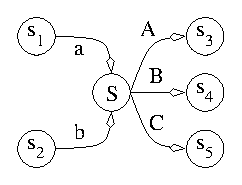
\includegraphics{./Fig3/trans.eps}

\item{\bf (1 pts.)} $a = b$.

\begin{tabular}{p{1.25in}p{1.25in}p{1.25in}}
a) Always  & b) Sometimes & c) Never  \\
\end{tabular}

\item{\bf (1 pts.)} $A = B = C$.

\begin{tabular}{p{1.25in}p{1.25in}p{1.25in}}
a) Always  & b) Sometimes & c) Never  \\
\end{tabular}

\item{\bf (1 pts.)} $a\  OR\  b = 1$.

\begin{tabular}{p{1.25in}p{1.25in}p{1.25in}}
a) Always  & b) Sometimes & c) Never  \\
\end{tabular}

\item{\bf (1 pts.)} $A\  OR\  B\  OR\  C = 1$.

\begin{tabular}{p{1.25in}p{1.25in}p{1.25in}}
a) Always  & b) Sometimes & c) Never  \\
\end{tabular}

\item{\bf (1 pts.)} $a\  AND\  b = 0$.

\begin{tabular}{p{1.25in}p{1.25in}p{1.25in}}
a) Always  & b) Sometimes & c) Never  \\
\end{tabular}

\item{\bf (1 pts.)} $A\  AND\  B\  AND\  C = 0$.

\begin{tabular}{p{1.25in}p{1.25in}p{1.25in}}
a) Always  & b) Sometimes & c) Never  \\
\end{tabular}


\pagebreak
For questions 21-23 use the algorithm and the corresponding piece 
of the control unit below.

\includegraphics[-60mm,50mm][0mm,51mm]{./Fig3/branch.eps}

\begin{verbatim}
if (x==1) then 
    if (y==1) then A=A+1;
    else           B=B+1;
else        
    if (y==1)      C=C+1;
    else           D=D+1;
\end{verbatim}
\vspace{16mm}


\item {\bf (3 pts.)} In which state does D get incremented?

\begin{tabular}{p{0.75in}p{0.75in}p{0.75in}p{0.75in}p{0.75in}}
a) S4 & b) S5 & c) S6 & d) S7 & e) other \\
\end{tabular}

\item {\bf (3 pts.)}Assume that X=1 and Y=1.  Given the partial timing 
diagram below, about what time will the outputs of the A register 
equal A+1?

\begin{tabular}{p{0.75in}p{0.75in}p{0.75in}p{0.75in}p{0.75in}}
a) 40nS & b) 60nS & c) 80nS & d) 120nS & e) 140nS \\
\end{tabular}

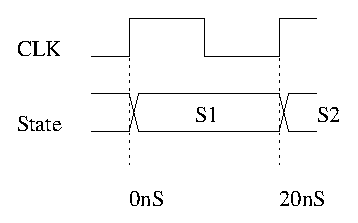
\includegraphics{./Fig3/time.eps}

\item {\bf (3 pts.)} How many states can the control unit be
reduced to, assuming that you keep state S1?

\begin{tabular}{p{0.75in}p{0.75in}p{0.75in}p{0.75in}p{0.75in}}
a) 1 & b) 4 & c) 5 & d) 6 & e) 7 \\
\end{tabular}

\pagebreak
Questions 24-54 {\bf (1 pt. each)}, questions 21-45 deal with the construction 
of a digital circuit to accomplish the task specified by the following 
algorithm.  A(0) refers to the LSB of A.  A$>>$ 1 refers to A shifted right 
1 bit.

{\small
\begin{verbatim}
while(1) {
    while(REQ == 0);              // If the control bit equals 0 or 00  mark A 
    A = datainA;                  // If the control bit equals 01       mark B 
    B = datainB;                  // If the control bit equals 10       mark C 
    ACK = 1;                      // If the control bit equals 1 or 11  mark D 
    while (REQ == 1);             // If the control bit is a don't care mark E 
    ACK = 0;
    C = 0;
    for (i=0; i<B; i++) {
        if (A(0) == 1) then
            C = C + 1;
        else 
            C = C - 1;
        A = A >> 1;
}   } 
\end{verbatim}}
\begin{figure}[ht]
\centerline{\psfig{figure=./Fig3/dp&cu.eps,width=5in,clip=}}
\end{figure}

\begin{tabular}{|l||l|l|l|l|l|l|l|}  \hline
State & ACK & A       & B      & C      & Mux        & count   & Add/Sub \\ \hline
      & 0   & 00 hold & 0 hold & 0 hold & 0 pass 0   & 00 hold & 0 add \\ \hline
      & 1   & 01 SR   & 1 load & 1 load & 1 pass C$\pm$1 & 01 down & 1 sub \\ \hline
      &     & 10 SL   &        &        &            & 10 up   &       \\ \hline
      &     & 11 load &        &        &            & 11 load &       \\ \hline   \hline
Wait1 & \x  &         &        &        &            &         &       \\ \hline
Get   & \x  &  \x     &  \x    &  \x    &  \x        &  \x     & \x    \\ \hline
Wait2 & \x  &  \x     &        &        &  \x        &  \x     &       \\ \hline
For/If &    &         &        &        &            &         &       \\ \hline
Inc   &     &  \x     &        &  \x    &  \x        &         & \x    \\ \hline
Dec   & \x  &         &        &  \x    &  \x        &         & \x    \\ \hline
Shift &     &  \x     &  \x    &  \x    &  \x        &         & \x    \\ \hline
\end{tabular}

\pagebreak
\item{\bf (3 pts.)} How many bits are in the status word?

\begin{tabular}{p{0.75in}p{0.75in}p{0.75in}p{0.75in}p{0.75in}}
a) 1 & b) 2 & c) 3 & d) 5 & e) 9 \\
\end{tabular}

\item{\bf (3 pts.)} How many bits are in the control word?

\begin{tabular}{p{0.75in}p{0.75in}p{0.75in}p{0.75in}p{0.75in}}
a) 2 & b) 3 & c) 5 & d) 7 & e) 9 \\
\end{tabular}

\item{\bf (3 pts.)} What is the Memory Input Equation for the For/If
flip flop; assume a ones-hot encoding?
\begin{description}
\item{a) } $D_{\rm For/If} = Q_{\rm Wait1}*L' + Q_{\rm Inc}*L*A(0) + Q_{\rm Dec}*L*A(0)'$
\item{b) } $Q_{\rm For/If} = D_{\rm Wait1}*L' + D_{\rm Inc}*L*A(0) + D_{\rm Dec}*L*A(0)'$
\item{c) } $D_{\rm For/If} = Q_{\rm Wait2}*REQ' + Q_{\rm Shift}$
\item{d) } $Q_{\rm For/If} = D_{\rm Wait2}*REQ' + D_{\rm Shift}$
\item{e) } None of the above.
\end{description}

\item{\bf (3 pts.)} Which of the following is the circuit playing in the
two-line handshake?
\begin{description}
\item{a) } Active Producer
\item{b) } Active Consumer
\item{c) } Passive Producer
\item{d) } Passive Consumer
\end{description}

\item{\bf (3 pts.)} The counter can be decremented in the For/If state.

\begin{tabular}{p{1.75in}p{1.75in}}
a) True  & b) False \\
\end{tabular}

\item {\bf (3 pts.)} Let A be N bits wide.  Let B's range be $[0,log_2(N)]$.
How many bits wide is the B register?

\begin{tabular}{p{1.30in}p{1.30in}p{2.00in}}
a) $log_2(log_2(N))$ & b) $log_2(log_2(N))+1$ &   \\
c) $log_2(N)$ & d) $log_2(N)+1$ & e) None of these.\\
\end{tabular}

\pagebreak
Questions 55,56 deal with the following figure.  Assume that the
setup, hold, and propagation delay of the flip flops is 2 nS.

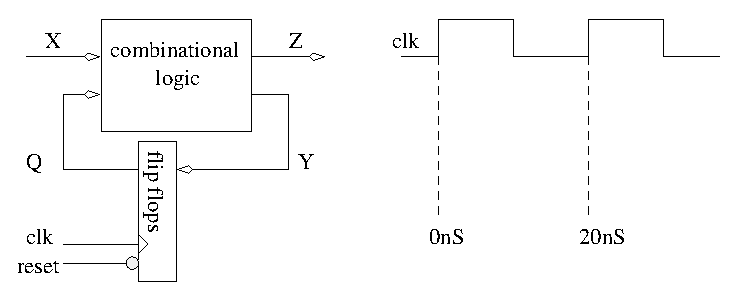
\includegraphics{./Fig3/fsm.eps}

\item {\bf (3 pts.)}Under what conditions will the flip flops be reset.
\begin{description}
\item{a) } When the clock rises and reset = 1.
\item{b) } When reset = 1.
\item{c) } When the clock rises and reset = 0.
\item{d) } When reset = 0.
\item{e) } None of the above.
\end{description}

\item {\bf (3 pts.)}At which of the following times does Q change?

\begin{tabular}{p{0.75in}p{0.75in}p{0.75in}p{0.75in}p{0.75in}}
a) 20nS  & b) 22nS  & c) 24nS & d) 26nS & e) 28nS \\
\end{tabular}

\pagebreak
%% This is an ABET survey
%% Edited 12/2005 to include program outcomes
%% Edited 12/2008 to remove program outcomes

%% \begin{center} 
%% CSE 271 -- Introduction to Digital Systems \\
%% Course Objectives Survey \\ 
%% Penn State Erie, The Behrend College
%% \end{center}

\small{
In order to assure the continued success of the Behrend ECE
program, I would appreciate your evaluation of whether or
not this course met its learning objectives.  All answers
will be kept anonymous and will be used for the future 
improvement of this course and the entire ECE program.
Please record your answers on the SCANTRON form.
Thanks for your help.
}

\begin{tabular}{p{0.25in}p{2.5in}|p{0.45in}|p{0.4in}|p{0.4in}|p{0.4in}|p{0.4in}|} \\ \cline{3-7}
    &  & 
{\scriptsize Strongly Disagree} A & 
{\scriptsize Disagree} B & 
{\scriptsize Neutral} C & 
{\scriptsize Agree} D & 
{\scriptsize Strongly Agree} E \\ \hline

\item & I understand how to convert numbers from one base to another and 
how to add and subtract numbers represented in binary and 2's complement 
form. 
 & & & & & \\ \hline

\item & I understand how to convert between a truth table, a circuit diagram,
boolean expression and a word statement.
 & & & & & \\ \hline

\item & I understand how to simplify logic expression into SOP or
POS minimal form with or without don't cares.
 & & & & & \\ \hline

\item & I understand how to use ESPRESSO to minimize combinational logic
functions.
 & & & & & \\ \hline

\item & I understand how adders, comparators, multiplexers and decoders 
are built and how they operate. 
 & & & & & \\ \hline

\item & I understand how D,T,SR,JK, latches, clock latches and flip flops 
are supposed to operate. 
 & & & & & \\ \hline

\item & I understand how registers, shift registers, counters, tri-state 
logic and RAMs are built and how they should operate. 
 & & & & & \\ \hline

\item & I understand how to design Finite State Machines using a dense 
or Ones Hot encoding. 
 & & & & & \\ \hline

\item & I understand how to implement complex digital systems using the 
datapath and control design approach. 
 & & & & & \\ \hline

\end{tabular}


\end{enumerate}

\end{document}


